\documentclass[a4paper]{article}

\usepackage{hyperref}
\usepackage{amsmath}
\usepackage{algorithmic}
\usepackage{algorithm}
\usepackage{graphicx}

\author{Paul van der Walt\footnote{\url{paul@@denknerd.org}}\\ \url{http://github.com/toothbrush/bsp-cg}}
\date{\today}
\title{A Parallel CG Algorithm\footnote{This work is inspired by Exercise 4.6 of PSC\cite{bisseling2004parallel}}}


\begin{document}

\maketitle

\begin{abstract}
    This is abstract
\end{abstract}

\newcommand{\ve}[1]{\ensuremath{\vec{#1}}}
\newcommand{\mat}[1]{\ensuremath{\boldsymbol{#1}}}
\newcommand{\plotsize}{0.7\textwidth}
\section{Introduction}

A well-known problem in problem in first-year courses on linear algebra is the question that
given some matrix \mat{A} and some vector \ve{b}, give \ve{x} such that the equation $\mat A \ve x = \ve b$ holds. A human would probably do Gaussian elimination, but
in scientific computing, a very widely used algorithm that comes to mind is the conjugate gradient method, which can iteratively compute the solution of a linear system of equations whose matrix is \emph{symmetric} and \emph{positive definite}.
As is well-known, a matrix is symmetric when $\mat A = \mat A^T$ holds, and positive definite is defined as the property that $\ve x^T \mat A \ve x > 0$, for all $\ve x \neq \ve 0$.

The conjugate gradient algorithm is given in Algorithm \ref{alg:seq-cg}, and is due to Hestenes and Stiefel \cite{hestenes1952methods}. It has been proven that the algorithm converges \cite{golub1996matrix}.

\begin{algorithm}
    \caption{Sequential conjugate gradient algorithm.}
\label{alg:seq-cg}
\begin{algorithmic}
    \REQUIRE ~\\
             $\mat A$ symmetric, positive definite, $n\times n$ matrix,\\
             $\ve  b$ vector of length $n$
    \ENSURE  $\mat A \ve x = \ve b$\\~\\
    \STATE $\ve x \leftarrow \ve{x_0}$ \COMMENT{initial guess}
    \STATE $k \leftarrow 0$ \COMMENT{iteration number}
    \STATE $\ve r \leftarrow \ve b - \mat A \ve x$
    \STATE $\rho \leftarrow ||\ve r||^2$
    \WHILE{$\sqrt{\rho} > \epsilon ||\ve b|| \wedge k < k_{max}$}
        \IF{$k=0$}
            \STATE $\ve p \leftarrow \ve r$
        \ELSE
            \STATE $\beta \leftarrow \rho/\rho_{old}$
            \STATE $\ve p \leftarrow \ve r + \beta \ve p$
        \ENDIF
        \STATE $\vec w \leftarrow \mat A \ve p$
        \STATE $\gamma \leftarrow \ve p . \ve w$
        \STATE $\alpha \leftarrow \rho/\gamma$
        \STATE $\ve x  \leftarrow \ve x + \alpha \ve p$
        \STATE $\ve r  \leftarrow \ve r - \alpha \ve w$
        \STATE $\rho_{old} \leftarrow \rho$
        \STATE $\rho   \leftarrow || \ve r || ^2$
        \STATE $k \leftarrow k+1$
    \ENDWHILE
\end{algorithmic}
\end{algorithm}


\section{The sequential algorithm}

To get a feel for the algorithm the first step was to implement a sequential version. The source code 

\section{The parallel algorithm}

\subsection{Complexity}

\subsection{Data distribution}

\section{Matrix generation}

% talk a bit about genmat.c

\section{Experimental results}

A number of experiments were done to explore what the effect of varying $p$,
$N$, nonzero density or processor distribution would be. Specifically, series
of matrices was generated to measure the running time with varying $p$ (section
\ref{sec:time-run}), running time with varying load imbalance (section
\ref{sec:imbalance-run}), and running time with varying $N$ (section
\ref{sec:nz-run}).

\subsection{Varying $p$}\label{sec:time-run}

\begin{figure}[h]
    \begin{center}
        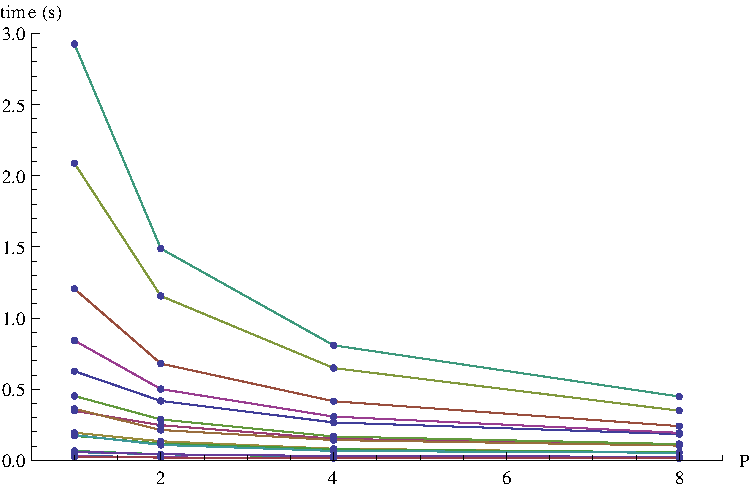
\includegraphics[width=\plotsize]{img/time-run.pdf}
    \end{center}
    \caption{Varying $P$ while keeping other factors constant.}
    \label{fig:time-run}
\end{figure}


\begin{figure}[h]
    \begin{center}
        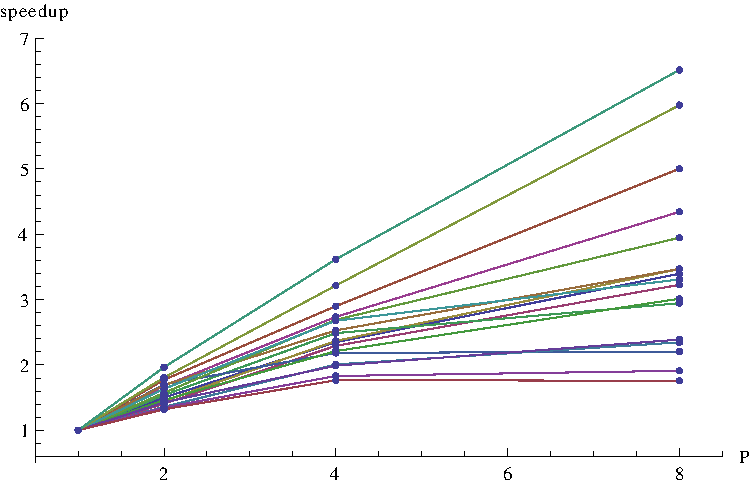
\includegraphics[width=\plotsize]{img/speedup.pdf}
    \end{center}
    \caption{The speedup achieved by increasing $P$ with various matrices.}
    \label{fig:speedup}
\end{figure}

\subsection{Varying load imbalance}\label{sec:imbalance-run}

\begin{figure}[h]
    \begin{center}
        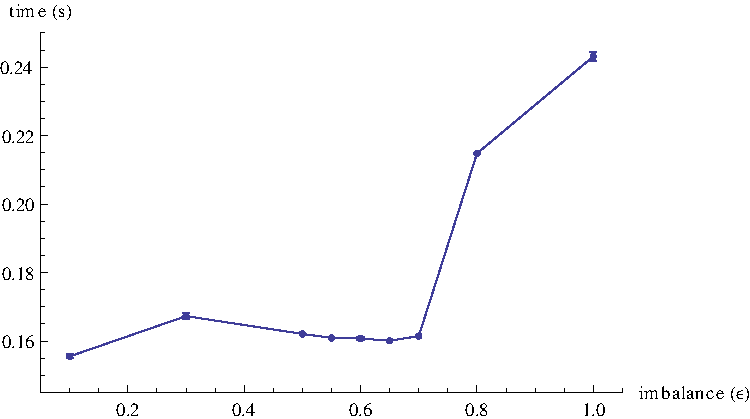
\includegraphics[width=\plotsize]{img/imbalance.pdf}
    \end{center}
    \caption{The load imbalance's effect on run time. $N=6000$, $P=8$, $\delta=0.1$}
    \label{fig:imbalance}
\end{figure}


\subsection{Varying $N$}\label{sec:nz-run}

\begin{figure}[h]
    \begin{center}
        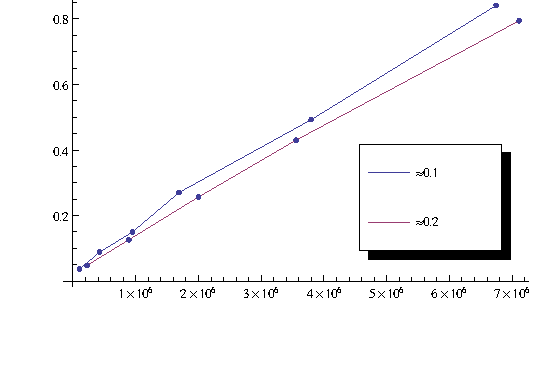
\includegraphics[width=\plotsize]{img/density-run.pdf}
    \end{center}
    \caption{Varying $N$ while achieving a constant final density. $P=2$}
    \label{fig:density-run}
\end{figure}

\section{Conclusion}


\appendix

\section{Bug fixed in BSPedupack}

After some experiments with the latest versions of BPSonMPI, OpenMPI and
BSPedupack, it became clear that there was a bug causing the parallel matrix-vector
multiplication function
\texttt{bspmv} to always return a zero-array (i.e. instead of the result vector
\texttt{u} containing the answer to the multiplication of some \texttt{A} and
\texttt{v}, it only contained zeroes), when run on a local Linux machine (the
problem didn't appear using the IBM compiler on Huygens).

The problem turned out to be that the function \texttt{bspmv} used
\texttt{bsp\_set\_tag\_size} with a second argument of type \texttt{int},
instead of \texttt{size\_t}, which BSPonMPI requires. When this had been
changed (no other changes to the code were necessary), the examples compiled
without warnings once again, and ran fine, producing the expected answers.

The surprising thing was that previously BSPedupack had functioned without
problems on my systems (Linux x86-64 and OS X), and it still worked on Huygens,
which probably means they have an older library somewhere, or that their
compiler (as opposed to my GNU CC compiler) is less strict in casting \texttt{size\_t} to \texttt{int} and vice versa.

The difference between \texttt{size\_t} and \texttt{int}, is that the former is
independent of the underlying architecture, while an \texttt{int} has a width
which depends on the processor's instruction size. Evidently the IBM compiler
is lenient and casts \texttt{int} to the struct \texttt{size\_t} without
problems, but the GNU CC compiler sets the value of the \texttt{size\_t} to 0.

%TODO add a diff

\section{Experimental data}

If one should want to duplicate the results found in this report, all that needs to be done
is to make a clone of the GitHub repository containing this project, which can be found at
\url{http://github.com/toothbrush/bsp-cg}. If one would like to try running the programs on the exact matrices
used to generate the results presented here, an archive containing all the matrices with their
different partitionings ($P=1,2,4,8, \ldots$) is provided (warning: large
download) at \url{http://denknerd.org/} %TODO provide matrices online

The archive contains a number of folders, which correspond to the various experimental runs
presented in this report. Each folder contains one or more \texttt{*.emm} files, which are the original
matrices as generated by \texttt{genmat}, and finally, the files \texttt{*.emm-$\left\{\texttt{P,u,v}\right\}n$} are
the output after having run Mondriaan on the \texttt{*.emm} file to partition the matrix for $n$ processors.



\section{Code listings}
% here we need
% the bspcg.c


\bibliographystyle{plain}
\bibliography{cg}
\end{document}
